\section{A Basic Arithmetic Logic Unit}

In Classical Computing and Digital Logic Design, the \textit{Arithmetic Logic Unit} (ALU) is a fundamental component of the \textit{Central Processing Unit} (CPU) of the computer 
that is responsible of carrying all of its the arithmetic and logical operations \cite{Giannakopoulos2015}. Depending on the design of the processor, an ALU can implement
a number of arithmetic or logical operations. An example set of arithmetic operations of an ALU may be: addition, subtraction, multiplication and division. We must note that
these are not the only ones. Many ALUs also implement boolean \textit{bitwise} operations, operations done between bits, like: AND, OR, NOT, XOR, Shift left and right.

At the other hand, an example of logical operation set of an ALU may be: Testing Equality/Inequality and Magnitude Comparison (Greater or Less than).

An ALU generally has two operand inputs, inputs that the ALU will operate upon, a Function or Operation code, a binary sequence that instructs the ALU to do the correct operation
with the given operand inputs and the Status input which is a bit sequence where each bit stands for a specific Status code or Status flag and its job is to note the status of the
last operation that was executed by the ALU. The two only outputs of the ALU are the Status output, essentially this output will wrap-around and update the Status register, and
the Ouput value where the product of the operation of the operands is stored. The diagram of this digital component is given in figure (2.8).

\begin{figure}[!ht]
    \centering
    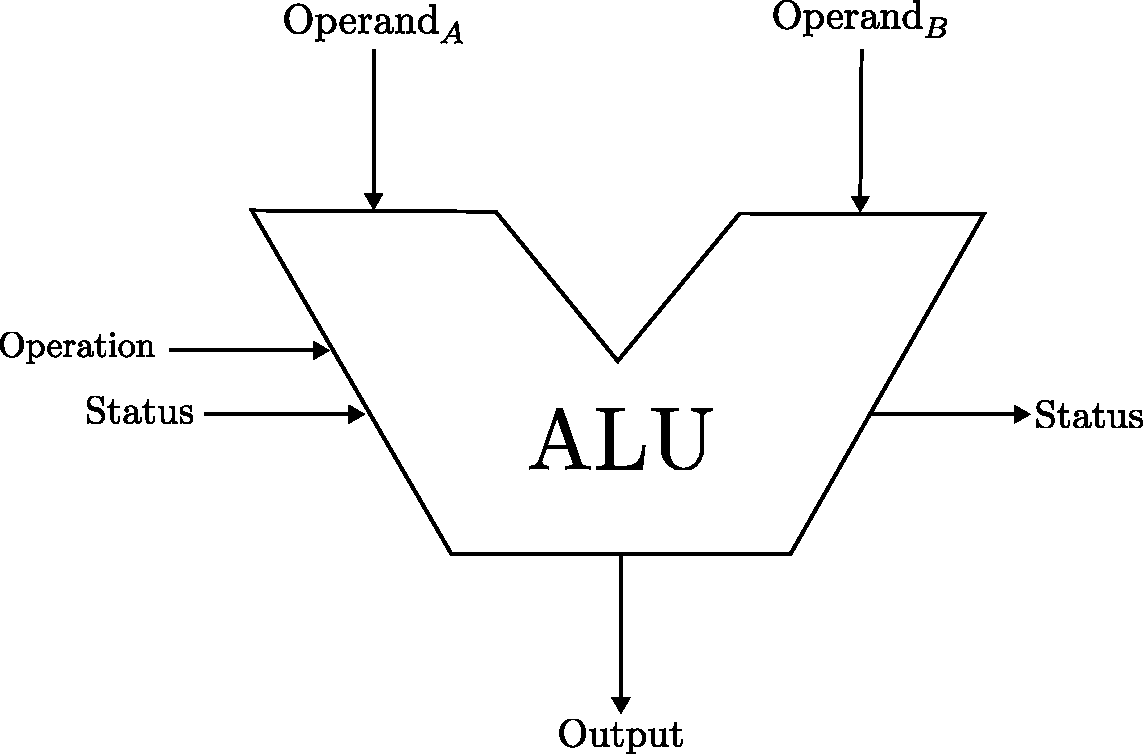
\includegraphics[scale=.4]{images/2_Classical_Computing/alu.pdf}
    \caption{The Arithmetic Logic Unit diagram}
\end{figure}

\newpage

We shall turn our attention now to the function/operation codes of the ALU. For a given number of implemented operations $n$, the ALU may need a bit-sequence of length:

\begin{equation}
    N_n=\lceil\log_2(n)\rceil
\end{equation}

So for $n=8$, eight operations, the ALU needs $N_8=\lceil\log_2(8)\rceil=3$ or a bit sequence of three bits wide. So we assign each operation to a binary number and we acquire the following table:

\begin{table}[!ht]
    \centering
    \begin{tabular}{c|c|c|c}
        Name & Function/Operation Code & Operation & Mnemonic Name\\
        \hline
        Addition        & $000$ & $A\leftarrow A+B$ & \verb|ADD|\\
        Subtraction     & $001$ & $A\leftarrow A-B$ & \verb|SUB|\\
        Multiplication  & $010$ & $A\leftarrow A\times B$ & \verb|MUL|\\
        Division        & $011$ & $A\leftarrow A\div B$ & \verb|DIV|\\
        Left Bit-Shift $B$-times  & $100$ & $A\leftarrow A<<B$ & \verb|LBS|\\
        Right Bit-Shift $B$-times & $101$ & $A\leftarrow A>>B$ & \verb|RBS|\\
        Test Equality   & $110$ & $A=B?$ & \verb|EQ|\\
        Test Magnitude  & $111$ & $A\geq B?$ & \verb|GTE|\\
    \end{tabular}
    \caption{An example function/operation code table for a basic Arithmetic Logic Unit}
\end{table}

For this kind of operation set we can also set which operation will interact with the Status register and update its flags. For example, the most logical pick may be
the \verb|EQ| and \verb|GTE| operations.

Following the above table we can schematically construct a very basic ALU:

\begin{figure}[ht]
    \centering
    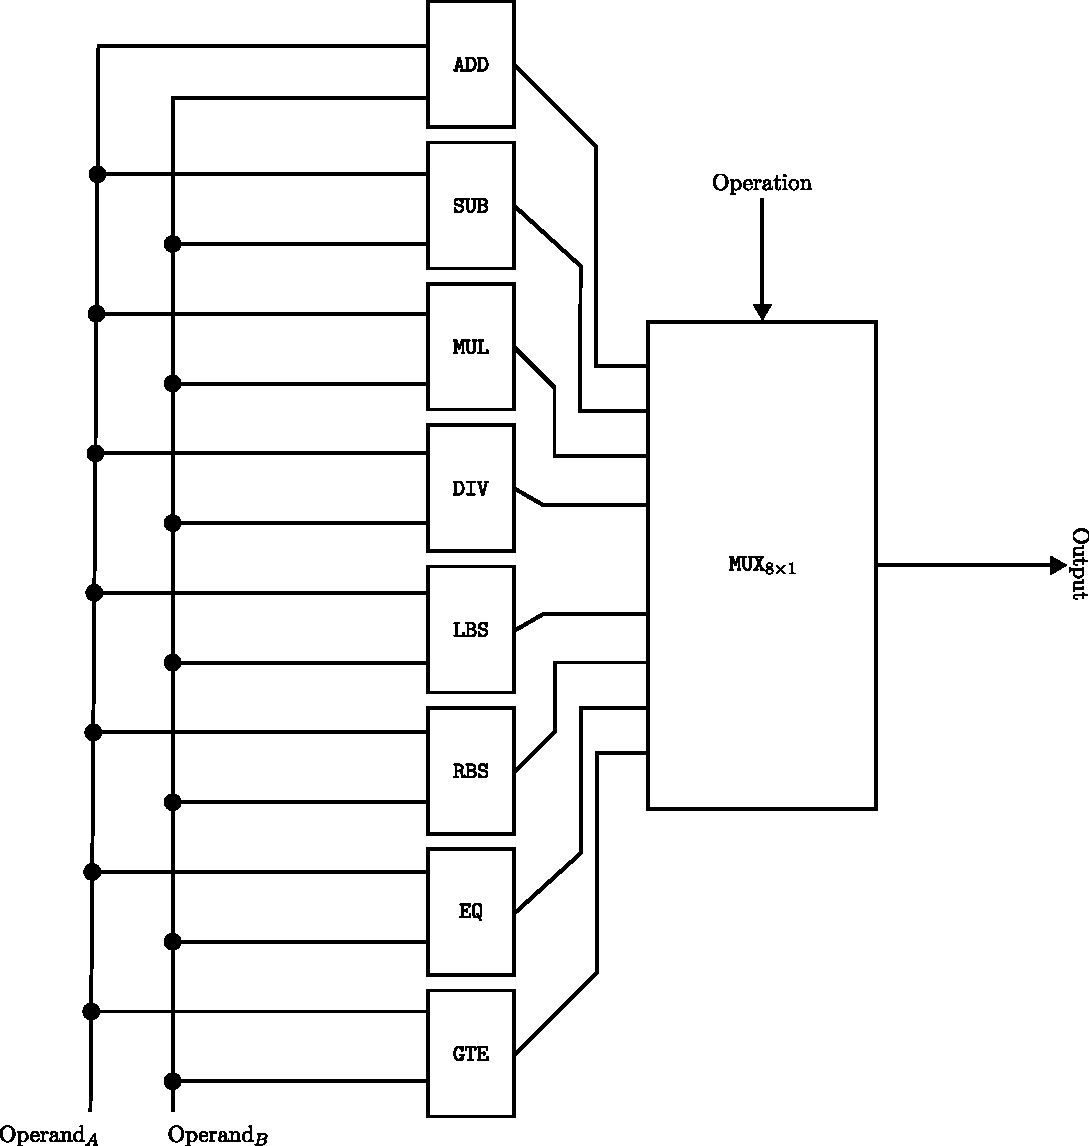
\includegraphics[scale=.6]{images/2_Classical_Computing/alu_design.pdf}
    \caption{A simple logic design of an example Arithmetic Logic Unit}
\end{figure}

The circuit in figure (2.9) computes all of the operations simultaneously but only outputs and/or updates the Status register when the appropriate Operationc
code is set, which is controlled by the \textit{multiplexer} circuit placed at the very end of the ALU's circuit.

We want to note that historically ALUs implement integer-based arithmetic operations. The unit that operates with real numbers encoded with a floating-point scheme, or
\textit{floating-point numbers}, is called the \textit{Floating-Point Unit}. This kind of units are fundamentally different and we will not analyze them further, since
they are out of the scope of this thesis.